\chapter{MM MPI}
In questo capitolo viene analizzato tutto quello che riguarda l'implementazione di MM MPI. La struttura del codice, le primitive MPI utilizzate, compilazione, esecuzioni, output dell'applicazione ed infine delle ottimizzazione per migliorare le prestazioni di MM MPI.

\section{Il codice dell'applicazione}
L'applicazione \`{e} scritta interamente in C ed utilizza la libreria mvapich2. Di seguito la lista dei file.

\begin{lstlisting}
contributors.txt
data
doc
logs
Makefile
Makefile.mm.dev
Makefile.mm.inc -> Makefile.mm.pg
Makefile.mm.pg
README
run_mm_mpi_dev.sh
run_mm_mpi_pg.sh
src
test.sh
\end{lstlisting}

La directory \textit{data} contiene i file di input da passare all'applicazione.

La directory \textit{doc} contiene i sorgenti di questa relazione

La directory \textit{src} contiene il codice dell'applicazione con i vari Makefile. Sia il codice che i Makefile verrano spiegati successivamente.

Nella root dell'applicazione ci sono poi vari script per l'esecuzione ed cosa molto importante il README con istruzioni su come compilare ed eseguire.

\subsection{Makefiles}
I Makefiles giocano un ruolo molto importante per la compilazione dell'applicazione. Di seguito il Makefile principale che \`{e} responsabile della compilazione delle varie versioni dell'applicazione.

\lstinputlisting{"../../Makefile"}

Ci sono poi dei Makefile secondari, uno per ogni versione dell'applicazione da compilare. Un esempio \`{e} il seguente:

\lstinputlisting{"../../src/cannon/Makefile.cblas"}

che compila la versione cblas di MM MPI. Nella riga 1 c'\`{e} l'inclusione di un altro file. Questo file contiene tutti i parametri per la corretta compilazione e differisce a seconda dell'ambiete di sviluppo. Per compilare ed eseguire MM MPI su un MBP i seguenti parametri sono stati utilizzati:

\lstinputlisting{"../../Makefile.mm.dev"}

Prima della compilazione dunque si deve creare il Makefile con i giusti parametri e poi creare un link simbolico \textit{Makefile.mm.inc}

\subsection{La directory src/}
Questa directory contiene tre sotto directory dove si possono trovare i file .c e .h che implementano MM MPI. Il codice \`{e} ben documentato con commenti (in inglese), dunque lascio all'utente l'esercizio di aprire i file sorgenti mentre legge la seguente relazione.

\subsubsection{src/shared}
In \textit{shared} si trovano funzioni che sono indipendenti dall'implementazione (seriale o parallela). Il contenuto \`{e} i seguente:

\begin{lstlisting}
format.c
format.h
reset.c
reset.h
shared.h
utils.c
utils.h
\end{lstlisting}

\textit{format.c} contiene funzioni accessorie per stampare i risultati sullo stdout e debug sullo stderr.

\textit{reset.c} contiene una funzione per fare il reset di una matrice: tutte le celle della matrice verranno impostate a 0.0.

L'unico contenuto di \textit{shared.h} \`{e} una variabile globale per controllare il debug dell'applicazione.

Infine \textit{utils.c} ha un parser degli argomenti passati da console: help, debug e file di input. C'\`{e} anche funzione per prendere il timestamp, utile per calcolare poi il tempo trascorso per la computazione (utilizzato solo per l'implementazione seriale).

\subsubsection{src/serial}
\textit{serial} contiene l'implementazione seriale della moltiplicazione. La lista dei file \`{e}:

\begin{lstlisting}
check.c
gendat.c
Makefile
mm.c
mxm.c
\end{lstlisting}

\textit{mm.c} contiene il main, dove tutto il flusso di lavoro viene guidato: dal parsing dei parametri passati da console, alla generazione dei dati per poi passare alla moltiplicazione vera e propria per poi concludere al controllo dei risultati, calcolo del tempo passato e la stampa allo stdout dei risultati.

\textit{mxm.c} contiente la vera moltiplicazione tra matrice: questa implementazione \`{e} la versione naive dell'algoritmo. Giusto per completezza, si riporta di seguito il codice:

\begin{lstlisting}
void mxm(int m, int l, int n, double a[][l], double b[][n],
         double c[][n]) {
    int     i, j, k;

    for (i = 0; i < m; i++) {
        for (j = 0; j < l; j++) {
            for (k = 0; k < n; k++) {
                c[i][k] += a[i][j] * b[j][k];
            }
        }
    }
}
\end{lstlisting}

Si ricorda che la sua complessit\`{a} \`{e} di $O(n^3)$.

Oltre al Makefile per guidare la compilazione, \textit{check.c} contiene una funzione per verificare se la moltiplicazione \`{e} avvenuta con successo e che abbia prodotto la C con i giusti risultati. Infine \textit{gendat.c} implementa una funzione per generare i dati delle matrici A e B.

Come ultima nota, nella sezione relativa all'esecuzione verr\`{a} spiegato il meccanismo che sta dietro alla generazione dei dati ed al relativo controllo del giusto risultato (che \`{e} uguale sia per l'implementazione seriale, sia per quella parallela).

\subsubsection{src/cannon}
La directory \textit{cannon} ha molti pi\`{u} file rispetto alla corrispettiva seriale. Questo perch\`{e} sono implementate varie versione ed ottimizzazioni che verrano spiegate dopo.

\begin{lstlisting}
check.c
gendat.c
Makefile
Makefile.cblas
Makefile.nonblock
Makefile.nonblock.cblas
Makefile.nonblock.openmp.inner
Makefile.nonblock.openmp.middle
Makefile.nonblock.openmp.nested
Makefile.nonblock.openmp.outer
Makefile.openmp.inner
Makefile.openmp.middle
Makefile.openmp.nested
Makefile.openmp.outer
mm.c
mxm.c
mxm-local.c
mxm-local.h
\end{lstlisting}

La lunga lista di Makefile serve a compilare queste diverse versioni dell'applicazione.

Come nella versione seriale troviamo sia \textit{check.c}, sia \textit{gendat.c} per\`{o} la loro implementazione \`{e} leggermente diversa. Il controllo viene fatto su un array invece che su un array di array mentre la generazione dei dati avviene utilizzando MPI: ogni nodo \`{e} responsabile di generare il proprio blocco di dati.

\textit{mm.c} ancora \`{e} il principale file dove il main guida tutto il flusso di lavoro: ci sono dei controlli preliminari da effettuare prima di prendere i dati dalla riga di comando. Il principale \`{e} controllare se il numero di processori che ho a disposizione sia un quadrato perfetto: se non lo fosse non potrei partizionare la matrice in blocchi per l'esecuzione parallela. Fatto ci\`{o}, si possono leggere i dati da console e iniziare a generare i dati delle matrici: qui c\'{e} un ulteriore controllo da fare. Si deve essere sicuri che le matrici siano "coperte" totalmente e senza scarti dal numero dei processori disponibili. Una volta passato questo controllo si prosegue alla generazione dei dati, moltiplicazione e controllo dei risultati: da notare che tutti questi passaggi sono effettuati tramite MPI. Se tutto dovesse andare bene, i risultato vengono diretti sullo stdout.

\textit{mxm.c} ha un'unica funzione che \'{e} responsabile di effettuare la moltiplicazione parallela sfruttando MPI e l'algoritmo di Cannon. Infatti in questa funzione \`{e} possibile distinguere le varie fasi dello stesso algoritmo.
Altra cosa da notare \'{e} la "doppia" implementazione: con la macro \textit{\#NONBLOCKING} si implementa un approccio non bloccante utilizzando primitive MPI non bloccanti ed un doppio buffer.

Infine \textit{mxm-local.c} implementa la moltiplicazione (seriale) tra sottoblocchi di matrice: il codice infatti viene eseguito su ogni processo e si occupa di moltiplicare solo i dati locali, indipendentemente dal contenuto degli altri nodi. Questo file inoltre contiene alcune ottimizzazioni per migliorare le prestazioni dell'intero algoritmo: infatti grazie ad alcune macro, si hanno ottimizziazioni OpenMP e CBlas.

\subsection{Primitive MPI utilizzate}
Per comprendere meglio l'implementazione parallela, si ha qui una lista di primitive utilizzate nell'applicazione. Per ogni primitiva si descrive l'interfaccia e l'utilizzo all'interno del codice.

\subsubsection{MPI\_Init}
\begin{lstlisting}
int MPI_Init( int *argc, char ***argv )
\end{lstlisting}
\begin{itemize}
  \item argc: puntatore al numero di argomenti
  \item argv: puntatore al vettore di argomenti
\end{itemize}

\textit{MPI\_Init} deve essere la prima istruzione ad essere chiamata prima di qualsiasi altra istruzione MPI. Si trova nel file \textit{mm.c} subito dopo le dichiarazioni di variabili. l'API \`{e}:

\subsubsection{MPI\_Comm\_size}
\begin{lstlisting}
int MPI_Comm_size( MPI_Comm comm, int *size )
\end{lstlisting}
\begin{itemize}
  \item comm: comunicatore MPI
  \item size: numero di processi nel gruppo del comunicatore (output)
\end{itemize}

\textit{MPI\_Comm\_size} determina la grandezza del gruppo associato al comunicatore. Si trova su 3 file: gendat.c, mm.c e mxm.c. Questo perch\`{e} tutti e tre i file hanno a che fare con operazioni MPI.

\subsubsection{MPI\_Comm\_rank}
\begin{lstlisting}
int MPI_Comm_rank( MPI_Comm comm, int *rank )
\end{lstlisting}
\begin{itemize}
  \item comm: comunicatore MPI
  \item rank: rank del processo chiamante nel gruppo del comunicatore (output)
\end{itemize}

Determina il rank del processo chiamante nel comunicatore. Come nel caso precedente, si trova su 3 file: gendat.c, mxm.c e mm.c. Sui primi due file \`{e} replicato due volte perch\`{e} vengono utilizzati due diversi comunicatori: quello generico (MPI\_COMM\_WORLD) ed un altro comunicatore con una topologia cartesiana, utilizzato per implementare l'algoritmo di Cannon.

\subsubsection{MPI\_Barrier}
\begin{lstlisting}
int MPI_Barrier( MPI_Comm comm )
\end{lstlisting}
\begin{itemize}
  \item comm: comunicatore
\end{itemize}

Blocca finch\`{e} tutti i processi nel comunicatore hanno raggiunto questa routine. Si trova solo sul file mm ed \`{e} utilizzato per sincronizzare i vari step dell'applicazione.

\subsubsection{MPI\_Wtime}
\begin{lstlisting}
double MPI_Wtime( void )
\end{lstlisting}

Ritorna il tempo trascorso del processo chiamante da un punto arbitrario nel passato. \`{E} utilizzato in mm.c per prendere il tempo prima e dopo la moltiplicazione parallela per poi calcolare il tempo trascorso.

\subsubsection{MPI\_Reduce}
\begin{lstlisting}
int MPI_Reduce(const void *sendbuf, void *recvbuf, int count, MPI_Datatype datatype, MPI_Op op, int root, MPI_Comm comm)
\end{lstlisting}
\begin{itemize}
  \item sendbuf: indirizzo del buffer da inviare
  \item recvbuf: indirizzo del buffer di ricezione, rilevante solo al processo root (output)
  \item count: numero di elementi in sendbuffer
  \item datatype: tipo di dati in sendbuf
  \item op: operazione di riduzione
  \item root: rank del processo root
  \item comm: comunicatore
\end{itemize}

La funzione \`{e} presente in mm.c e serve a ridurre gli output della funzione check() distribuiti tra i nodi ad un solo valore. La funzione \`{e} cos\`{i} chiamata:

\begin{lstlisting}
MPI_Reduce(&local_check,   // Indirizzo del buffer da inviare
           &ok,            // Indirizzo del buffer ricevente
           1,              // Numero di elementi
           MPI_INTEGER,    // Tipologia di elementi
           MPI_SUM,        // L'operazione da effettuare (somma)
           0,              // Rank del processo root
           MPI_COMM_WORLD);// Comunicatore
\end{lstlisting}

Si ricorda che se check() ritorna 0, il check \`{e} andato a buon fine. Dunque si sommano tutti i check distribuiti e si memorizzano in "ok". Questa variabile verr\`{a} controllata in seguito per verificare se la moltiplicazione ha avuto successo.

\subsubsection{MPI\_Cart\_create}
\begin{lstlisting}
int MPI_Cart_create(MPI_Comm comm_old, int ndims, const int dims[], const int periods[], int reorder, MPI_Comm *comm_cart)
\end{lstlisting}
\begin{itemize}
  \item comm\_old: comunicatore in input
  \item ndims: numero di dimensioni della griglia cartesiana
  \item dims: array di ndims interi per specificare il numero di processi in ogni dimensione
  \item periods: array di ndims valori per specificare se la griglia \`{e} peiodica (true) o meno (false) in ogni dimensione
  \item reorder: il ranking pu\`{o} essere riordinato o meno
  \item comm\_cart: comunicatore con la nuova topologia cartesiana
\end{itemize}

La funzione \`{e} utilizzata per creare un comunicatore con topologia cartesiana ed \`{e} presente sia in gendat.c che in mxm.c. L'unica differenza tra le due chiamate \`{e} che in gendat.c non si ha bisogno della periodicit\`{a} della griglia mentre in mxm.c si: questo perch\`{e} in mxm.c la griglia deve essere shiftata con wraparound, proprio come l'algoritmo di Cannon.

\subsubsection{MPI\_Cart\_coords}
\begin{lstlisting}
int MPI_Cart_coords(MPI_Comm comm, int rank, int maxdims, int coords[])
\end{lstlisting}
\begin{itemize}
  \item comm: comunicatore
  \item rank: rank del processo nel gruppo di comm
  \item maxdims: lunghezza del vettore coords
  \item coords: array di interi (lunghezza di ndims) contenente le coordinate cartesiane del processo specificato (output)
\end{itemize}

Determina le coordinate del process nella topolgia cartesiana dato uno specifico rank nel gruppo. \`{E} utilizzata sia in gendat.c, sia in mxm.c: le coordinate sono fondamentali per capire la posizione virtuale del blocco di dati nello spazio cartesiano.

\subsubsection{MPI\_Cart\_shift}
\begin{lstlisting}
int MPI_Cart_shift(MPI_Comm comm, int direction, int disp, int *rank_source, int *rank_dest)
\end{lstlisting}
\begin{itemize}
  \item comm: comunicatore con struttura cartesiana
  \item direction: la coordinata della dimensione da shiftare
  \item disp: movimento (> 0: shift in alto, < 0 shift in basso)
  \item rank\_source: rank del processo sorgente (output)
  \item rank\_dest: rank del processo destinazione (output)
\end{itemize}

Ritorna i sorgenti e destinazioni shiftati data una direzione ed un numero di shift. La funzione \`{e} utilizzata solo in mxm.c, ovvero il file dove l'algoritmo di Cannon \`{e} implementato: necessito di questa primitiva per effettuare l'allineamento iniziale e finale.

\subsubsection{MPI\_Sendrecv\_replace}
\begin{lstlisting}
int MPI_Sendrecv_replace(void *buf, int count, MPI_Datatype datatype, int dest, int sendtag, int source, int recvtag, MPI_Comm comm, MPI_Status *status)
\end{lstlisting}
\begin{itemize}
  \item buf: indirizzo iniziale del buffer da inviare e per ricevere (output)
  \item count: numero di elementi nel buffer
  \item datatype: tipo di elementi nel buffer
  \item dest: rank di destinazione
  \item sendtag: tag per il messaggio da inviare
  \item source: rank sorgennte
  \item recvtag: tag per il messaggio da ricevere
  \item comm: comunicatore
  \item status: oggetto status (output)
\end{itemize}

La funzione invia e riceve dati utilizzando un singolo buffer in maniera bloccante. \`{E} presente solo in mxm.c ed invia/riceve blocchi di matrice ai/dai blocchi adiacenti per implementare l'algoritmo di Cannon utilizzando il comunicatore con topologia cartesiana.

\subsubsection{MPI\_Isend}
\begin{lstlisting}
int MPI_Isend(const void *buf, int count, MPI_Datatype datatype, int dest, int tag, MPI_Comm comm, MPI_Request *request)
\end{lstlisting}
\begin{itemize}
  \item buf: indirizzo del buffer da inviare
  \item count: numero di elementi contenuti nel buffer
  \item datatype: tipo di dati contenuti nel buffer
  \item dest: rank di destinazione
  \item tag: tag del messaggio
  \item comm: comunicatore
  \item request: richiesta di comunicazione (output)
\end{itemize}

La funzione implementa un invio non bloccante: questo vuol dire che ritorna anche se il messaggio non \`{e} stato inviato. \`{E} utilizzata in mxm.c nella versione non bloccante utilizzando un doppio buffer.

\subsubsection{MPI\_Irecv}
\begin{lstlisting}
int MPI_Irecv(void *buf, int count, MPI_Datatype datatype, int source, int tag, MPI_Comm comm, MPI_Request *request)
\end{lstlisting}
\begin{itemize}
  \item buf: indirizzo del buffer da ricevere
  \item count: numero di elementi contenuti nel buffer
  \item datatype: tipo di dati contenuti nel buffer
  \item dest: rank sorgente
  \item tag: tag del messaggio
  \item comm: comunicatore
  \item request: richiesta di comunicazione (output)
\end{itemize}

La funzione implementa una ricezione non bloccante: questo vuole dire che ritorna anche sel il messaggio non \`{e} stato ricevuto. \`{E} utilizzato in mxm.c nella versione non bloccante utilizzando un doppio buffer.

\subsubsection{MPI\_Waitall}
\begin{lstlisting}
int MPI_Waitall(int count, MPI_Request array_of_requests[], MPI_Status array_of_statuses[])
\end{lstlisting}
\begin{itemize}
  \item count: lunghezza della lista
  \item array\_of\_requests: array di richieste
  \item array\_of\_statuses: array di status (output)
\end{itemize}

La funzione aspetta che tutte le request passate abbiano terminato. La primitiva \`{e} utilizzata in mxm.c nella versione non bloccante e serve per bloccare l'esecuzione fino a che ogni gli shift a sinistra ed in alto abbiano finito.

\subsubsection{MPI\_Comm\_free}
\begin{lstlisting}
int MPI_Comm_free(MPI_Comm *comm)
\end{lstlisting}
\begin{itemize}
  \item comm: comunicatore
\end{itemize}

La primitiva marca il comunicatore pronto per essere deallocato. Questo significa che il comunicatore non \`{e} pi\`{u} necessario. Presente sia in gendat.c ed mxm.c per deallocare il comunicatore con topologia cartesiana.

\subsubsection{MPI\_Finalize}
\begin{lstlisting}
int MPI_Finalize( void )
\end{lstlisting}

Termina l'ambiente di esecuzione MPI ed \`{e} presente solo in mm.c, il file responsabile del setup dell'ambiente MPI. Dopo questa primitiva nessun comando MPI pu\`{o} essere chiamato a meno che un altro ambiente MPI sia configurato.

\section{Compilazione}

La compilazione di MM MPI \`{e} guidata da una serie di Makefile. Prima della compilazione si deve creare il file \textit{Makefile.mm.inc} oppure creare un link simbolico ad uno dei file gi\`{a} presenti.
Una volta che il file \textit{Makefile.mm.inc} esiste, \`{e} possibile lanciare il comando \textit{make}. Se non si passa nessun argomento, make compiler\`{a} tutte le possibili variazioni di MM MPI: una versione seriale e dodici versioni parallele.
Se si vuole compilare solo la versione di Cannon non bloccante ottimizzata con cblas, baster\`{a} digitare:

\begin{lstlisting}
$ make 2D-cannon-nonblock-cblas
\end{lstlisting}

I binari prodotti inizieranno con \textit{x.mm\_} seguiti dalla implementazione. La lista completa dei binari \`{e}:

\begin{lstlisting}
$ ls x.mm_*
x.mm_2D_cannon
x.mm_2D_cannon_cblas
x.mm_2D_cannon_nonblock
x.mm_2D_cannon_nonblock_cblas
x.mm_2D_cannon_nonblock_openmp_inner
x.mm_2D_cannon_nonblock_openmp_middle
x.mm_2D_cannon_nonblock_openmp_nested
x.mm_2D_cannon_nonblock_openmp_outer
x.mm_2D_cannon_openmp_inner
x.mm_2D_cannon_openmp_middle
x.mm_2D_cannon_openmp_nested
x.mm_2D_cannon_openmp_outer
x.mm_serial
\end{lstlisting}

\section{Esecuzione}

Prima di spiegare come eseguire MM MPI, \`{e} dovereso spiegare come la generazione dei dati ed il controllo funzionano.

\subsubsection{Data file}
MM MPI prende in input un file di testo con il seguente formato

\begin{lstlisting}
$ cat data/2_repititions
4 4 4 2
8 8 8 2
16 16 16 2
32 32 32 2
64 64 64 2
128 128 128 2
192 192 192 2
256 256 256 2
384 384 384 2
512 512 512 2
768 768 768 2
1024 1024 1024 2
1536 1536 1536 2
2048 2048 2048 2
3072 3072 3072 2
4096 4096 4096 2
\end{lstlisting}

Il formato del file \`{e} il seguente:

\begin{lstlisting}
M   L   N   #repitizioni
\end{lstlisting}

dove la matrice A ha dimensioni MxL, la matrice B ha dimensioni LxN. In questo modo \`{e} sempre possibile effettuare la moltiplicazione. L'ultimo parametro indica il numero di volte che la moltiplicazione deve essere effettuata senza rigenerare i dati. Nell'esempio precedente vediamo che tutte le matrici generate sono quadrate di dimensione n e che la moltiplicazione verr\`{a} ripetuta 2 volte.
La ripetizione \`{e} molto importante soprattutto quando si vogliono collezionare dati e si vuole attenuare eventuale rumore durante gli esperimenti.

\subsubsection{Generazione delle matrici A e B}

Le matrici A e B vengono generate come nella figura \ref{fig:matrix_gen}. Sia A sia B sono matrici quadrate di dimensioni 4.

La matrice A ha tutte le righe uguali ed ogni cella ha il valore dell'i-esima colonna +1. L'ultima colonna contiene sempre il valore di L nel file precedente.

La matrice B invece ha tutte le colonne uguali ed ogni cella contiene numero dell'i-esima riga + 1 che divide 1 ($\frac{1}{i+1}$). La prima riga ha sempre 1 mentre l'ultima riga contiene sempre $\frac{1}{N}$

\begin{figure}[htbp]
    \begin{center}
        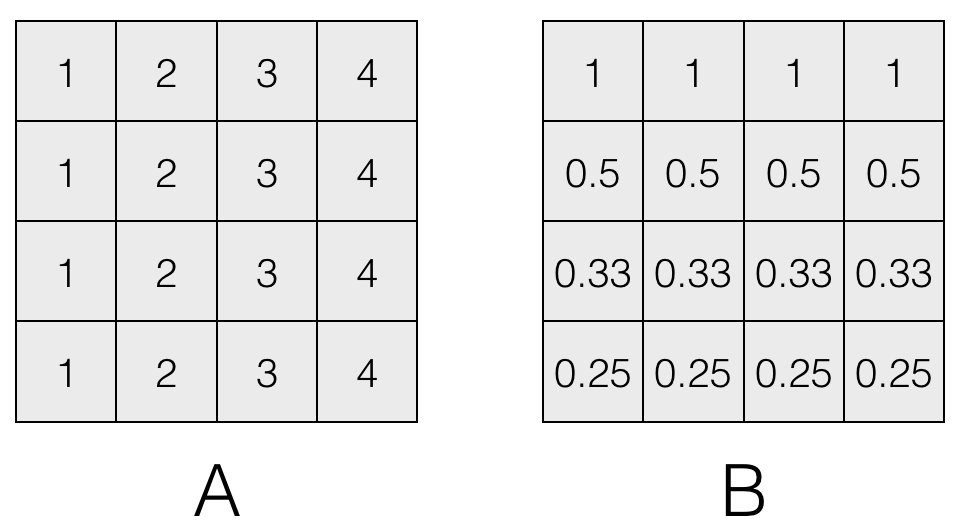
\includegraphics[width=8cm]{immagini/matrix_gen.png}
    \end{center}
    \caption{Generazione delle matrici A e B}
    \label{fig:matrix_gen}
\end{figure}

La generazione delle matrici parallele \`{e} un po' pi\`{u} complessa perch\`{e} le matrici sono rappresentate in un array e distribuite su diversi nodi.
Per quanto riguarda la matrice A:

\begin{lstlisting}
a[i * L_DBLOCK + j] = (double)((coordinates[1] * L_DBLOCK) + j + 1);
\end{lstlisting}

\begin{itemize}
  \item i: valore nel M\_DBLOCK
  \item j: valore nel L\_DBLOCK
  \item L\_DBLOCK: larghezza del blocco L
  \item coordinates[1]: valore della colonna nelle coordinate cartesiane
\end{itemize}

Per quanto riguarda la matrice B:

\begin{lstlisting}
b[i * N_DBLOCK + j] = 1.0 / (double)((coordinates[0] * L_DBLOCK) + i + 1);
\end{lstlisting}

\begin{itemize}
  \item i: valore nel L\_DBLOCK
  \item j: valore nel N\_DBLOCK
  \item N\_DBLOCK: larghezza del blocco N
  \item coordinates[0]: valore della riga nelle coordinate cartesiane
\end{itemize}

\subsubsection{Controllo della matrice finale}

Le matrici cos\`{i} generate producono un risultato prevedibile come mostrato in figura \ref{fig:matrix_gen_multiplication}. Il risultato oltre che prevedibile \`{e} anche facile da verificare. La matrice C infatti avr\`{a} in ogni cella il valore L.

\begin{figure}[htbp]
    \begin{center}
        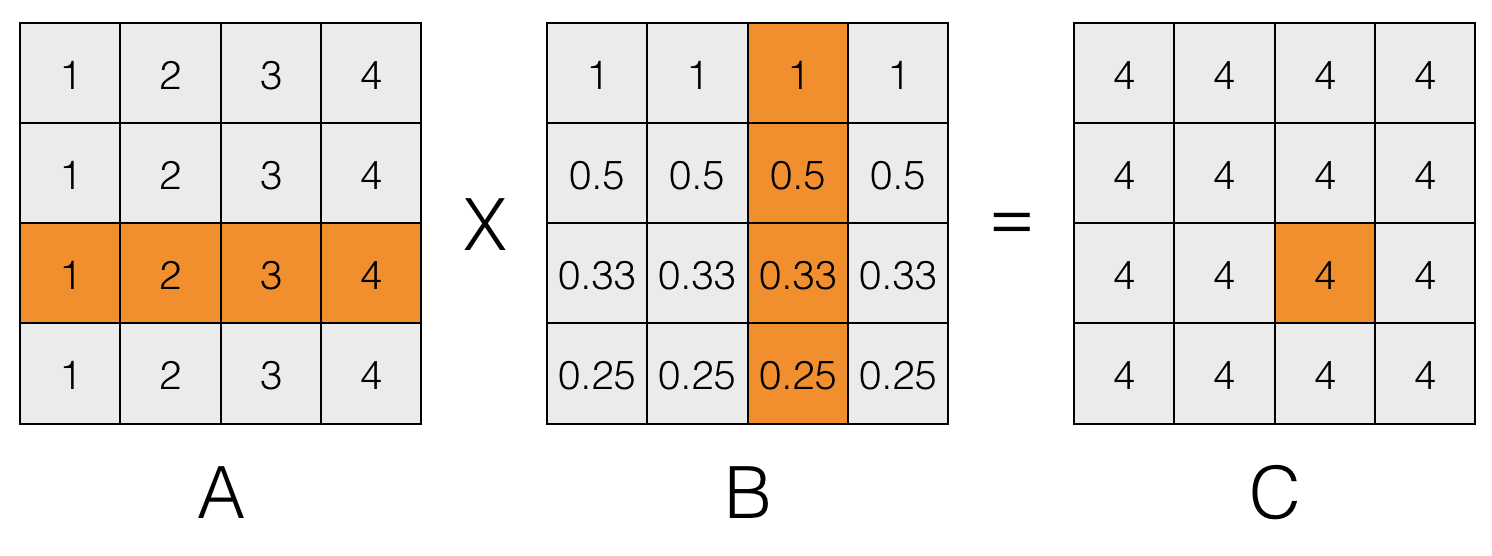
\includegraphics[width=10cm]{immagini/matrix_gen_multiplication.png}
    \end{center}
    \caption{Moltiplicazione delle matrici A e B}
    \label{fig:matrix_gen_multiplication}
\end{figure}

Ora si hanno tutti gli elementi per eseguire l'applicazione.

\subsubsection{Esecuzione seriale}

La versione seriale \`{e} la pi\`{u} semplice da eseguire.

\begin{lstlisting}
./x.mm_serial -f data/demo_data
\end{lstlisting}

Dove \textit{demo\_data} \`{e} il file contenente le informazioni per effettuare la moltiplicazione.

\subsubsection{Esecuzione parallela su singola macchina}

Se si vuole testare la versione MPI senza avere a disposizione il cluster, lo si pu\`{o} fare attraverso \textit{mpirun}

\begin{lstlisting}
mpirun -n 16 ./x.mm_2D_cannon -f data/demo_data
\end{lstlisting}

In questo caso sto eseguendo la versione standard di Cannon utilizzando 16 processi.

\subsubsection{Esecuzione parallela su cluster}

L'esecuzione sul cluster \`{e} leggermente un pochino pi\`{u} complessa rispetto alle altre.

\begin{lstlisting}
$ PROC_NAME=x.mm_2D_cannon
$ qsub -lnodes=8:ppn=2,mem=9050mb -d . -N $PROC_NAME -e logs -o logs -v EXE=$PROC_NAME,DATA=example_data run_mm_mpi_pg.sh
\end{lstlisting}

Il job \`{e} sottomesso utilizzando qsub specificando che si ha bisogno di 8 nodi con 2 processori e un utilizzo totale di 9GB di memoria.\textit{-d} specifica l'area di lavoro, \textit{-N} il nome del processo, \textit{-e/-o} la directory dove i log verranno memorizzati ed infine \textit{-v} specifica la lista di variabili da passare allo script \textit{run\_mm\_mpi\_pg.sh} che le utilizzer\`{a} per eseguire MM MPI.

\lstinputlisting{"../../run_mm_mpi_pg.sh"}

Notare che le variabili \textit{\$PBS\_NODEFILE} \textit{\$PBS\_NP} sono impostate in automatico da Torque.

\section{Debug output}

Il debug dell'applicazione puo\`{o} essere attivato attraverso l'opzione "-d". Il debug sar\`{a} differente a seconda della versione seriale e parallela: la versione parallela ha informazioni addizionali quali il rank del processo, le inforamzioni relative alla topologia cartesiana ed ai relativi shift.

\begin{lstlisting}
[diego@cgcw mm_mpi]$ ./x.mm_serial -f data/demo_data  -d
Executing ./x.mm_serial
Generating data for matrix A[4 x 4]
[function: gendat] a[0][0] = 1
[function: gendat] a[0][1] = 2
[function: gendat] a[0][2] = 3
[function: gendat] a[0][3] = 4
[function: gendat] a[1][0] = 1
[function: gendat] a[1][1] = 2
[function: gendat] a[1][2] = 3
[function: gendat] a[1][3] = 4
[function: gendat] a[2][0] = 1
[function: gendat] a[2][1] = 2
[function: gendat] a[2][2] = 3
[function: gendat] a[2][3] = 4
[function: gendat] a[3][0] = 1
[function: gendat] a[3][1] = 2
[function: gendat] a[3][2] = 3
[function: gendat] a[3][3] = 4
Generating data for matrix B[4 x 4]
[function: gendat] b[0][0] = 1
[function: gendat] b[0][1] = 1
[function: gendat] b[0][2] = 1
[function: gendat] b[0][3] = 1
[function: gendat] b[1][0] = 0.5
[function: gendat] b[1][1] = 0.5
[function: gendat] b[1][2] = 0.5
[function: gendat] b[1][3] = 0.5
[function: gendat] b[2][0] = 0.333333
[function: gendat] b[2][1] = 0.333333
[function: gendat] b[2][2] = 0.333333
[function: gendat] b[2][3] = 0.333333
[function: gendat] b[3][0] = 0.25
[function: gendat] b[3][1] = 0.25
[function: gendat] b[3][2] = 0.25
[function: gendat] b[3][3] = 0.25
Matrix C will be [4 x 4]
Let's do the math (1 repetitions)
mm: Matrix-matrix multiply test C(m,n) = A(m,l)*B(l,n)
-------------------------------------------------------
      Problem size     |            |            |    |
   m   |   l   |   n   |  Time (s)  |  (Gflop/s) | OK |
-------------------------------------------------------
      4|      4|      4|      0.0000|  4.2667e-02|  T |
-------------------------------------------------------
\end{lstlisting}

L'output fornisce tutte le informazioni necessare per eseguire il debug dell'applicazione.
Per quanto riguarda l'esecuzione su cluster il debug viene rediretto su stderr, dunque contenuto nel file di errore.

\begin{lstlisting}
[function: gendat, MPI rank: 0] My coordinates are: 0, 0
[function: gendat, MPI rank: 0] BLOCKS - M: 2 L: 2 N: 2
[function: gendat, MPI rank: 0] A[0 * 2 + 0]: 0 * 2 + 0 + 1 = 1
[function: gendat, MPI rank: 0] A[0 * 2 + 1]: 0 * 2 + 1 + 1 = 2
[function: gendat, MPI rank: 0] A[1 * 2 + 0]: 0 * 2 + 0 + 1 = 1
[function: gendat, MPI rank: 0] A[1 * 2 + 1]: 0 * 2 + 1 + 1 = 2
[function: gendat, MPI rank: 0] B[0 * 2 + 0]: 1.0 / ((0 * 2) + 0 + 1) = 1
[function: gendat, MPI rank: 0] B[0 * 2 + 1]: 1.0 / ((0 * 2) + 0 + 1) = 1
[function: gendat, MPI rank: 0] B[1 * 2 + 0]: 1.0 / ((0 * 2) + 1 + 1) = 0.5
[function: gendat, MPI rank: 0] B[1 * 2 + 1]: 1.0 / ((0 * 2) + 1 + 1) = 0.5
[function: mxm, MPI rank: 0] My coordinates are: 0, 0
[function: mxm, MPI rank: 0] Left rank: 1, Up rank: 2
[function: mxm, MPI rank: 0] Initial matrix alignment for A: shift of 0 to 0
[function: gendat, MPI rank: 1] My coordinates are: 0, 1
[function: gendat, MPI rank: 1] BLOCKS - M: 2 L: 2 N: 2
[function: gendat, MPI rank: 1] A[0 * 2 + 0]: 1 * 2 + 0 + 1 = 3
[function: gendat, MPI rank: 1] A[0 * 2 + 1]: 1 * 2 + 1 + 1 = 4
[function: gendat, MPI rank: 1] A[1 * 2 + 0]: 1 * 2 + 0 + 1 = 3
[function: gendat, MPI rank: 1] A[1 * 2 + 1]: 1 * 2 + 1 + 1 = 4
[function: gendat, MPI rank: 1] B[0 * 2 + 0]: 1.0 / ((0 * 2) + 0 + 1) = 1
[function: gendat, MPI rank: 1] B[0 * 2 + 1]: 1.0 / ((0 * 2) + 0 + 1) = 1
[function: gendat, MPI rank: 1] B[1 * 2 + 0]: 1.0 / ((0 * 2) + 1 + 1) = 0.5
[function: gendat, MPI rank: 1] B[1 * 2 + 1]: 1.0 / ((0 * 2) + 1 + 1) = 0.5
[function: mxm, MPI rank: 1] My coordinates are: 0, 1
[function: mxm, MPI rank: 1] Left rank: 0, Up rank: 3
[function: mxm, MPI rank: 1] Initial matrix alignment for A: shift of 0 to 1
[function: gendat, MPI rank: 2] My coordinates are: 1, 0
[function: gendat, MPI rank: 2] BLOCKS - M: 2 L: 2 N: 2
[function: gendat, MPI rank: 2] A[0 * 2 + 0]: 0 * 2 + 0 + 1 = 1
[function: gendat, MPI rank: 2] A[0 * 2 + 1]: 0 * 2 + 1 + 1 = 2
[function: gendat, MPI rank: 2] A[1 * 2 + 0]: 0 * 2 + 0 + 1 = 1
[function: gendat, MPI rank: 2] A[1 * 2 + 1]: 0 * 2 + 1 + 1 = 2
[function: gendat, MPI rank: 2] B[0 * 2 + 0]: 1.0 / ((1 * 2) + 0 + 1) = 0.333333
[function: gendat, MPI rank: 2] B[0 * 2 + 1]: 1.0 / ((1 * 2) + 0 + 1) = 0.333333
[function: gendat, MPI rank: 2] B[1 * 2 + 0]: 1.0 / ((1 * 2) + 1 + 1) = 0.25
[function: gendat, MPI rank: 2] B[1 * 2 + 1]: 1.0 / ((1 * 2) + 1 + 1) = 0.25
[function: mxm, MPI rank: 2] My coordinates are: 1, 0
[function: mxm, MPI rank: 2] Left rank: 3, Up rank: 0
[function: mxm, MPI rank: 2] Initial matrix alignment for A: shift of -1 to 3
[function: gendat, MPI rank: 3] My coordinates are: 1, 1
[function: gendat, MPI rank: 3] BLOCKS - M: 2 L: 2 N: 2
[function: gendat, MPI rank: 3] A[0 * 2 + 0]: 1 * 2 + 0 + 1 = 3
[function: gendat, MPI rank: 3] A[0 * 2 + 1]: 1 * 2 + 1 + 1 = 4
[function: gendat, MPI rank: 3] A[1 * 2 + 0]: 1 * 2 + 0 + 1 = 3
[function: gendat, MPI rank: 3] A[1 * 2 + 1]: 1 * 2 + 1 + 1 = 4
[function: gendat, MPI rank: 3] B[0 * 2 + 0]: 1.0 / ((1 * 2) + 0 + 1) = 0.333333
[function: gendat, MPI rank: 3] B[0 * 2 + 1]: 1.0 / ((1 * 2) + 0 + 1) = 0.333333
[function: gendat, MPI rank: 3] B[1 * 2 + 0]: 1.0 / ((1 * 2) + 1 + 1) = 0.25
[function: gendat, MPI rank: 3] B[1 * 2 + 1]: 1.0 / ((1 * 2) + 1 + 1) = 0.25
[function: mxm, MPI rank: 0] Initial matrix alignment for B: shift of 0 to 0
[function: mxm, MPI rank: 0] Iterate through 2 dimensions
[function: mxm, MPI rank: 1] Initial matrix alignment for B: shift of -1 to 3
[function: mxm, MPI rank: 3] My coordinates are: 1, 1
[function: mxm, MPI rank: 3] Left rank: 2, Up rank: 1
[function: mxm, MPI rank: 3] Initial matrix alignment for A: shift of -1 to 2
[function: mxm, MPI rank: 1] Iterate through 2 dimensions
[function: mxm, MPI rank: 1] A: Sending data to 0, Receiving data from 0
[function: mxm, MPI rank: 1] B: Sending data to 3, Receiving data from 3
[function: mxm, MPI rank: 2] Initial matrix alignment for B: shift of 0 to 2
[function: mxm, MPI rank: 2] Iterate through 2 dimensions
[function: mxm, MPI rank: 2] A: Sending data to 3, Receiving data from 3
[function: mxm, MPI rank: 3] Initial matrix alignment for B: shift of -1 to 1
[function: mxm, MPI rank: 3] Iterate through 2 dimensions
[function: mxm, MPI rank: 3] A: Sending data to 2, Receiving data from 2
[function: mxm, MPI rank: 0] A: Sending data to 1, Receiving data from 1
[function: mxm, MPI rank: 0] B: Sending data to 2, Receiving data from 2
[function: mxm, MPI rank: 0] A: Sending data to 1, Receiving data from 1
[function: mxm, MPI rank: 2] B: Sending data to 0, Receiving data from 0
[function: mxm, MPI rank: 1] A: Sending data to 0, Receiving data from 0
[function: mxm, MPI rank: 1] B: Sending data to 3, Receiving data from 3
[function: mxm, MPI rank: 1] Final matrix alignment for A: shift of 0 to 1
[function: mxm, MPI rank: 1] Final matrix alignment for B: shift of 1 to 3
[function: mxm, MPI rank: 2] A: Sending data to 3, Receiving data from 3
[function: mxm, MPI rank: 2] B: Sending data to 0, Receiving data from 0
[function: mxm, MPI rank: 2] Final matrix alignment for A: shift of 1 to 3
[function: mxm, MPI rank: 2] Final matrix alignment for B: shift of 0 to 2
[function: mxm, MPI rank: 3] B: Sending data to 1, Receiving data from 1
[function: mxm, MPI rank: 3] A: Sending data to 2, Receiving data from 2
[function: mxm, MPI rank: 3] B: Sending data to 1, Receiving data from 1
[function: mxm, MPI rank: 3] Final matrix alignment for A: shift of 1 to 2
[function: mxm, MPI rank: 3] Final matrix alignment for B: shift of 1 to 1
[function: mxm, MPI rank: 0] B: Sending data to 2, Receiving data from 2
[function: mxm, MPI rank: 0] Final matrix alignment for A: shift of 0 to 0
[function: mxm, MPI rank: 0] Final matrix alignment for B: shift of 0 to 0
\end{lstlisting}

La prima cosa che si nota \`{e} la verbosit\`{e} del debug. La versione parallela contiene molte pi\`{u} informazioni rispetto alla corrispettiva parallela. Altra cosa da notare \`{e} la non linearit\`{a} delle informazioni che si hanno: MPI esegue codice su diversi nodi/macchine e non assicura ovviamente un'esecuzione perfettamente sincronizzata.

\section{Ottimizzazioni}

MM MPI ha due implementazioni di base: la versione seriale e quella parallela. Ci sono poi una serie di ottimizzazioni sulla versione parallela per migliorare le performance di esecuzione.

\subsection{MPI non bloccante}

La prima ottimizzazione \`{e} a livello MPI. La versione standard di MM MPI utilizza \textit{MPI\_Sendrecv\_replace} che ha un comportamento bloccante: questo significa che fino a che le copie non sono state effettuate la funzione non ritorna. Inoltre la funzione utilizza un solo buffer per inviare e ricevere dati e questo potrebbe rappresentare un collo di bottiglia per quanto riguarda le comunicazioni.

Si \`{e} provato a superare questo problema utilizzando due chiamate non bloccanti utilizzando un doppio buffer. La sezione di codice che lo implementa \`{e} la seguente:

\begin{lstlisting}
// Shift matrix A left by one
MPI_Isend(a_buf[i % 2], A_DBLOCK, MPI_DOUBLE, left, 1, comm_2d, &request_handles[0]);
MPI_Irecv(a_buf[(i + 1) % 2], A_DBLOCK, MPI_DOUBLE, right, 1, comm_2d, &request_handles[1]);
debug_printf(__func__, rank, "A: Sending data to %i, Receiving data from %i\n", left, right);

// Shift matrix B up by one
MPI_Isend(b_buf[i % 2], B_DBLOCK, MPI_DOUBLE, up, 1, comm_2d, &request_handles[2]);
MPI_Irecv(b_buf[(i + 1) % 2], B_DBLOCK, MPI_DOUBLE, down, 1, comm_2d, &request_handles[3]);
debug_printf(__func__, rank, "B: Sending data to %i, Receiving data from %i\n", up, down);

// Let's wait all the shifts/communications to happen
MPI_Waitall(4, request_handles, status_handles);
\end{lstlisting}

a\_buf e b\_buf sono due array cos\`{i} definti:

\begin{lstlisting}
a_buf[0] = a;
a_buf[1] = (double *)malloc(A_DBLOCK * sizeof(double));

b_buf[0] = b;
b_buf[1] = (double *)malloc(B_DBLOCK * sizeof(double));
\end{lstlisting}

cos\`{i} da avere un doppio buffer, uno per l'invio di dati ed uno per la ricezione di dati. In questo modo le operazioni di invio e di ricezione sono completamente indipendenti l'una dall'altra.

\subsection{Moltiplicazione con OpenMP}

Le altre due ottimizzazioni invece sono a livello di moltipicazioni tra matrici. La prima, OpenMP va a parallelizzare l'algoritmo seriale della moltiplicazioni tra matrici. L'algoritmo seriale ha 3 cicli for annidati e si \`{e} provato a parallelizzarli in diversi modi: sul ciclo esterno, su quello centrale, su quello interno e su quello interno e centrale insieme. Si \`{e} cos\`{i} generato 4 versioni per l'implementazione bloccante e 4 per l'implementazione non bloccante.

Un estratto di codice dell'ottimizzazione del ciclo esterno:

\begin{lstlisting}
    // The parallel pragma starts a parallel block
    // By default data are shared
    // t, k, j are private, so just i is shared
    // the scheduler is automatic: the compiler will pick up the best one
#pragma omp parallel for default(shared) private(t,k,j) schedule(auto)
    for (i = 0; i < m; i++) {
        for (j = 0; j < l; j++) {
            t = a[i * l + j];
            for (k = 0; k < n; k++) {
                c[i * n + k] = c[i * n + k] + t * b[j * n + k];
            }
        }
    }
\end{lstlisting}

La regola gnerale di OpenMP \`{e} che tutte le variabili in uno scope esterno sono condivise di default nella regione parallela. Tutte le variabili in sola lettura dovrebbero essere condivise mentre le variabili che scrivo dovrebber essere locali e marcate come private.

\subsection{Moltiplicazione con CBLAS dgemm}

L'ultima ottimizzazione \`{e} l'utilizzo di CBLAS dgemm per la moltiplicazione delle sottomatrici. Questo sostituisce completamente i 3 cicli for annidati con la seguente chiamata:

\begin{lstlisting}
cblas_dgemm(CblasRowMajor, CblasNoTrans, CblasNoTrans, m, n, l, 1.0, a, l, b, n, 1.0, c, n);
\end{lstlisting}

\begin{itemize}
  \item CblasRowMajor: indica che le matrici sono memorizzate riga x colonna
  \item CblasNoTrans: indica che le matrici A e B non devono essere trasposte prima della moltiplicazione
  \item m, n, l: interi che indicano le grandezze delle matrici: A[m x l], B[l x n], C[m x n]
  \item alpha: valore reale per scalare il prodotto delle matrici A e B
  \item a: matrice A
  \item l: numero di colonne in A
  \item b: matrice B
  \item n: numero di colonne in B
  \item alpha: valore reale per scalare la matrice C
  \item c: matrice C
  \item n: numero di colonne di C
\end{itemize}

Questa ottimizzazione genera due versioni di MM MPI: una per la versione bloccante ed una per la versione non bloccante


In totale si hanno 12 versioni di MM MPI:
\begin{itemize}
    \item 1 versione seriale
    \item 1 versione parallela (senza ottimizzazioni)
    \item 8 versioni di OpenMP (4 bloccanti e 4 non bloccanti)
    \item 2 versioni cblas (1 bloccante ed una non bloccante)
\end{itemize}

Nel prossimo capitolo verranno analizzate le performance di tutte le versioni su diversi input.
